\chapter{Project Documentation}
% --------------------------------------%
\section{Project Plan}
\subsection{Project Overview}
The goal of this project is to create and organize a lab, which shows and explains future students of the Ostschweizer Fachhochschule (OST) how reverse engineering is performed and which tactics are used to get information out of a program. To accomplish this task, the lab will have several exercises organized in the different domains. These exercises will be accessible through the Hacking-Lab website. 

\subsubsection*{Hand-In}
The finished report will be handed in according to the rules set by the "Studiengangsleitung Informatik" and the supervisor:
\begin{itemize}
    \item The PDF version will be sent to the advisor and to the OST archive.
    \item The printed version will be handed in to the supervisor for reading and grading.
\end{itemize}

\subsection{Management}
\subsubsection*{Time Management}
The project started on the first week of the semester (KW 38) and ends in week 51 giving us around 14 weeks to be done with the Hand-In. \\
Since the module has a total ECTS of 8 each of the students has to work around 240h during the semester which can be seen in table \ref{time_ects} together with the total planned time investment. This means, that per week each student should work around 17.1 hours.

\begin{table}
    \centering
    \begin{tabular}{||c c c c||} 
        \hline
        Name & ECTS & Time spent per Week [h] & Total Time spent [h]\\ [0.5ex] 
        \hline\hline
        Gianluca Nenz & 8 & 17.1 & 240 \\ 
        \hline
        Ronny Mueller & 8 & 17.1 & 240 \\
        \hline
        Thomas Kleb & 8 & 17.1 & 240 \\ 
        \hline
        \textbf{Total} & 32 & 52.3 & 720 \\[1ex] 
        \hline
    \end{tabular}
    \caption{Time Investments}
    \label{time_ects}
\end{table}

\subsubsection*{Planning and Project Management}
In the past modules Software Engineering Practices (SEP) 1 and 2  we were introduced to different ways to plan and organize a project. The main tools we learned, Rational Unified Process (RUP) and Scrum, are mainly used in software development but can be adapted to other projects aswell. They both use different aspects of time management and organisation which is why we intend to apply them to our project. \\
We use RUP to section our project into Inception, where we get a first insight into the project and how we want it to resolve; Elaboration, to plan our project, define the workload-distribution and setting up first concepts of the finished labs; The construction phase is mainly used to plan, build and test the labs while the last phase, the transition phase, is used as buffer and to finish our product. \\ 
To make sure everything works as planned we use Scrum with its sprints to setup milestones and tasks which help structurize the development. 

\subsection{Organisation}

\subsubsection*{Participants}
The "Studienarbeit"-Team consists of three students: Gianluca Nenz, Ronny Muel\-ler and Thomas Kleb. The work on the project and documentation will be evenly distributed between these three participants. Bigger decisions are made as a team in either the meetings with or without the advisor (the advisor will be notified on any change made).

\subsubsection*{Advisor}
The teams advisor for the "Studienarbeit" is Ivan Buetler who is teaching cybersecurity modules at the OST.

\subsubsection*{Division of Labor}
The project has multiple facets that need to be taken care of. This is why the team has decided to distribute the work load between the three. This doesn't mean that the work is done by only the chosen student but rather that he is the one responsible that it works as planned.
\begin{table}[H]
    \begin{tabular}[t]{||p{4cm}||}
        \hline
        Gianluca Nenz \\
        \hline\hline
        Sprint Meetings \\ 
        \hline
        Lab 3: x64dbg \\
        \hline
        Lab 4: ASM - Refresher \\ 
        \hline
        Lab 6: Dynamic - debug\\
        \hline
        Lab 8: UN-PW\\[1ex] 
        \hline
    \end{tabular}
    \hfill
    \begin{tabular}[t]{||p{4cm}||}
        \hline
        Ronny Mueller \\
        \hline\hline
        Meeting Notes \\
        \hline
        Lab 1: IDA \\ 
        \hline
        Lab 5: Static-debug \\
        \hline
        Lab 7: First Reversing Attempts \\ 
        \hline
        Lab 11: Patching\\[1ex] 
        \hline
    \end{tabular}
    \hfill
    \begin{tabular}[t]{||p{4cm}||}
        \hline
        Thomas Kleb \\
        \hline\hline
        Testing \\ 
        \hline
        Documentation \\
        \hline
        Lab 2: GDB \\ 
        \hline
        Lab 9: Pwntools\\
        \hline
        Lab 10: AES\\[1ex] 
        \hline
    \end{tabular}
    \caption{Work Distribution per Student}
    \label{work_dis}
\end{table}

\subsection{Planning and Milestones}

\subsubsection*{Phases and Iterations}
The project is comprised of the four steps of RUP. Each of those phases has multiple iterations which create the different sprints for the project. The meetings with the advisor will be on thursdays while the team meetings will be held tuesdays. Each iteration / sprint will be of a seven day length.

\noindent We started the "Studienarbeit" before we began with the regular school. In the week before we each made research and plans about the upcoming project. After having a talk with the advisor it was decided to first find out the level of knowledge each student has to allow easier planning for the advisor.
\begin{table}[H]
    \centering
    \begin{tabular}{|p{0.12\linewidth}|p{0.15\linewidth}|p{0.15\linewidth}|p{0.46\linewidth}|}
        \hline
        \multicolumn{4}{||c||}{\textbf{Inception}} \\
        \hline \hline
        Iteration & Start & End & Description \\
        \hline \hline
        0 & 12.09.2022 & 18.09.2022 & Collection of ideas and planning first meeting\\
        \hline
        1 & 19.09.2022 & 25.09.2022 & First meeting and handout of exercises to assess the knowledge of the students \\
        \hline
        2 & 26.09.2022 & 02.10.2022 & Working on the exercises and receiving solutions for harder ones \\
        \hline
    \end{tabular}
    \caption{RUP: Inception Phase Planning}
    \label{inception_table}
\end{table}

\noindent The elaboration phase is used to plan and assess the possible risks in this project. This consists of a documentation structure, the project plan and the risk management to make sure the construction phase has no major hickups.
\begin{table}[H]
    \centering
    \begin{tabular}{|p{0.12\linewidth}|p{0.15\linewidth}|p{0.15\linewidth}|p{0.46\linewidth}|}
        \hline
        \multicolumn{4}{||c||}{\textbf{Elaboration}} \\
        \hline \hline
        Iteration & Start & End & Description \\
        \hline \hline
        3 & 03.10.2022 & 09.10.2022 & First big meeting with advisor; Creating project plan and risk analysis.\\
        \hline
        4 & 10.10.2022 & 13.10.2022 & Project plan and documentation is set; Problem domains and learn concepts are defined \\
        \hline
        5 & 14.10.2022 & 25.10.2022 & Lab concepts are defined \\
        \hline
    \end{tabular}
    \caption{RUP: Elaboration Phase Planning}
    \label{elaboration_table}
\end{table}

\noindent The construction phase is where the labs are primarily built. 
\begin{table}[H]
    \centering
    \begin{tabular}{|p{0.12\linewidth}|p{0.15\linewidth}|p{0.15\linewidth}|p{0.46\linewidth}|}
        \hline
        \multicolumn{4}{||c||}{\textbf{Construction}} \\
        \hline \hline
        Iteration & Start & End & Description \\
        \hline \hline
        6 & 21.10.2022 & 01.11.2022 & POC for static and dynamic challenge; started testing \\
        \hline
        7 & 01.11.2022 & 08.11.2022 & Lab static and dynamic finished; POC First RE Attempts and UN-PW with testing \\
        \hline
        8 & 08.11.2022 & 15.11.2022 & Finishing lab UN-PW and RE Attempts; POC Pwntool lab \\
        \hline
        9 & 15.11.2022 & 22.11.2022 & Introduction labs, AES and testing \\
        \hline
        10 & 22.11.2022 & 29.11.2022 & POC patching lab and assembly lab \\
        \hline
        11 & 29.11.2022 & 06.12.2022 & Internal testing of all labs finished; all labs complete\\
        \hline
    \end{tabular}
    \caption{RUP: Construction Phase Planning}
    \label{construction_table}
\end{table}

\noindent To make sure enough time is planned a buffer week was added to the transition phase. This phase is also mainly used to finish up the documentation and implement the different challenges to Hacking Lab. The last week is used to clean up and hand in the documentation and abstract to both the OST and the advisor.
\begin{table}[H]
    \centering
    \begin{tabular}{|p{0.12\linewidth}|p{0.15\linewidth}|p{0.15\linewidth}|p{0.46\linewidth}|}
        \hline
        \multicolumn{4}{||c||}{\textbf{Transition}} \\
        \hline \hline
        Iteration & Start & End & Description \\
        \hline \hline
        12 & 06.12.2022 & 13.12.2022 & Documentation completion \\
        \hline
        13 & 13.12.2022 & 20.12.2022 & Finalizing documentation \\
        \hline
        14 & 20.12.2022 & 23.12.2022 & Preparing for hand-In \\
        \hline
    \end{tabular}
    \caption{RUP: Transition Phase Planning}
    \label{transition_table}
\end{table}

\subsubsection*{Milestones}
To guarantee the success of the project milestones were defined with a deadline.

\begin{table}[H]
    \centering
    \begin{tabular}[]{|| p{5cm} | c | p{6.2cm} ||}
        \hline
        Milestones & Deadline & Description \\
        \hline \hline
        M1 - Solving RE Exercises & 05.10.2022 & The Team tries to solve the given exercises to find the level of RE knowledge. \\
        \hline
        M2 - Defining problem domains and learn concepts& 13.10.2022 & Problem domains are defined, first learn concepts are planned \\
        \hline
        M3 - Lab Concepts & 25.10.2022 & Lab Concepts are defined to start working on the construction. \\
        \hline
        M4 - Setup Labs & 06.12.2022 & Labs are setup and tested. \\
        \hline
        M5 - Hand-In & 23.12.2022 & Document is handed in to the advisor and OST \\
        \hline
    \end{tabular}
    \caption{Milestones set for the project}
    \label{milestones_table}
\end{table}

\subsubsection*{Time Tracking}
For time tracking the team has decided on using a third party application named Clockify \cite{clockify}. To have an overview on what the team spents its time on we decided to create different tags: 
\begin{itemize}
    \item Documentation: Working on the documentation
    \item GitLab: Maintaining the infrastructure of the repositories
    \item Meetings: Sprint- and advisormeetings
    \item Preparation: Research before the start of the project
    \item RE-Labs: Creating the different labs
    \item Research: Researching for the labs
    \item Testing: Testing the labs with different volunteers
\end{itemize}

\subsubsection*{Issue Tracking}
The issue tracking is done on GitLabs own interface to have as few difficulties as possible. To have an easier overview of the different issues the team has created tags to differentiate between the issues and their assigned student. 



\subsubsection*{GANTT Diagram}

\begin{figure}[H]
    \centering
    \begin{sideways}
    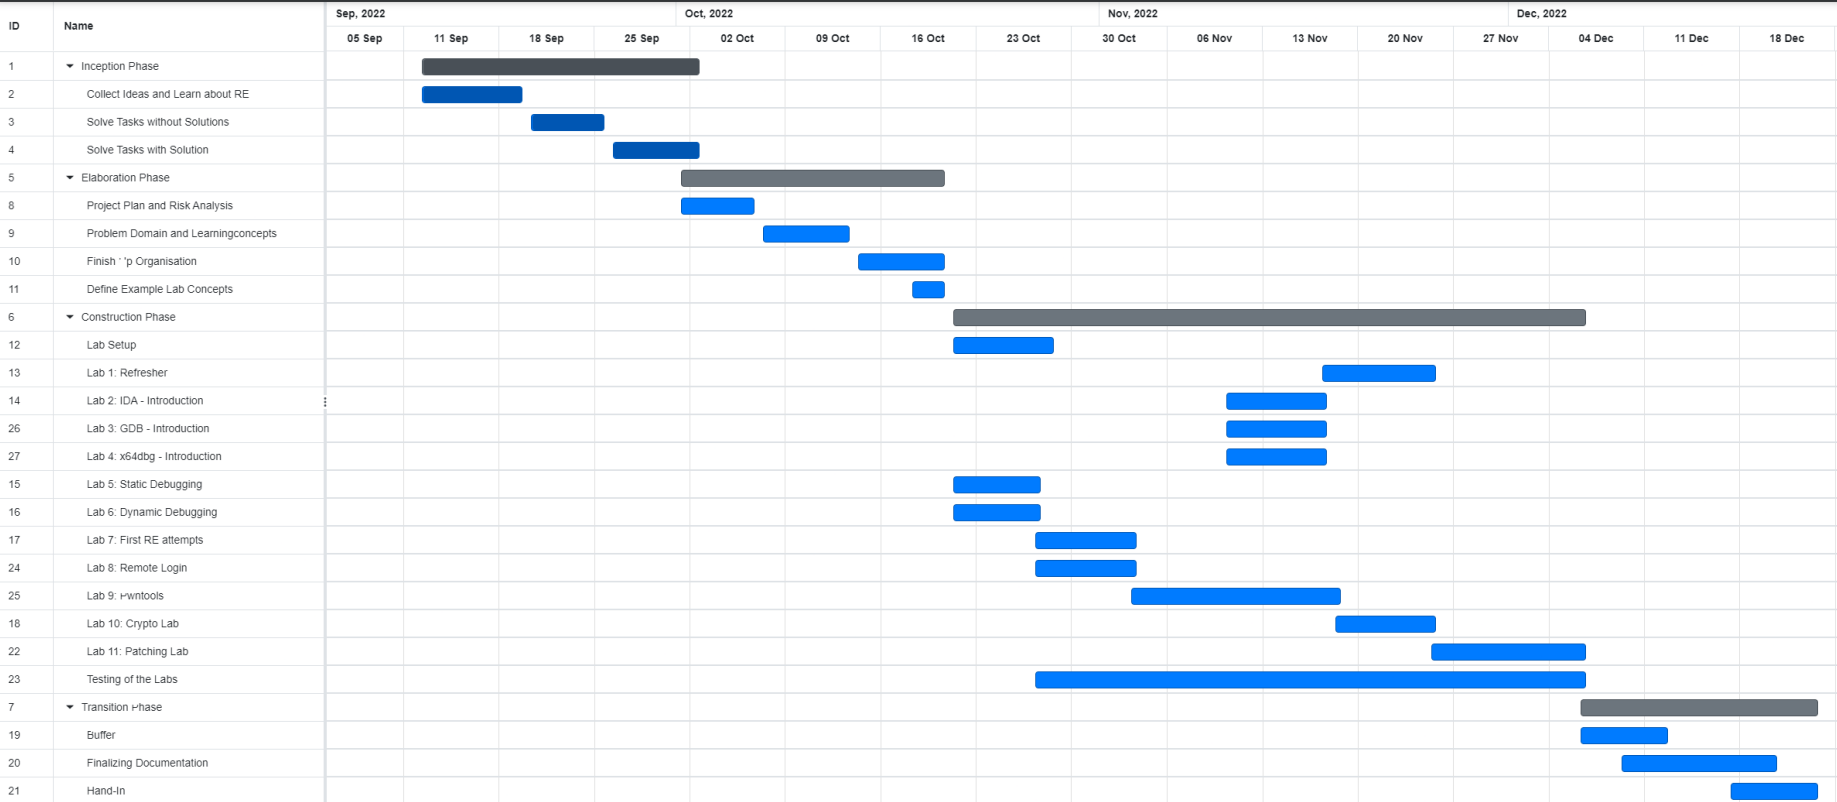
\includegraphics[width=600pt, height=380pt]{resources/gantt.png}
    \end{sideways}
    \caption{GANTT chart}
    \label{gantt_figure}
\end{figure}



\subsubsection*{Meetings}
The team has meetings each tuesday to elaborate problems and check up on the progress. These meetings are also used to distribute the work load. \\
On Thursdays the team meets the advisor Ivan Buetler to inform him on the progress done and the problems that came up. These meetings have different time schedules to fit everyones calender. \\
Each meeting will be documented and uploaded to the GIT repository. After each meeting the participants should know what to do and how to contact each other if any problems arise.

%\subsubsection*{CI/CD}

\subsubsection*{Projectmanagment}
The whole project will use a GitLab repository. To make sure no confusion happens a multirepo principle is used where one repository is only for the documentation and protocols and the other one is for code, information gathered, etc. Each student works on a branch and creates a merge request where the other students check the proposed changes for errors and when nothing is found, they merge the changes. 

\subsection{Testing}
This chapter describes how the quality of the challenges was determined and the feedback was evaluated. \\
The labs were tested by many different participants. This testing was done to ensure the challenges were solvable and understandable for the intended purpose. The testing can be divided into two parts.

\subsubsection{Internal Tests}
After every challenge was completed and uploaded to the Hacking-Lab platform, the creator checked the challenge again. After the creator finished his testing, he signaled the other students from the group to test the challenge. Any questions, mistakes or feedback from these tests were immediately reported to the creator. He then decided which parts he had to change. Additionally at the next supervisor meeting the challenge was presented and the supervisor was also able to give feedback to the challenge.

\subsubsection{Testing with third-party students}
In order to get realistic feedback from students, we asked cyber security students in their fifth semester to solve the labs and provide feedback. This feedback was collected using Google Forms. This tool allows to create simple surveys, which can then be analyzed in graphs automatically. \\
Only some of the challenges were solved by this group. The feedback received was helpful. However, since many of these students were also busy with a SA, it was a bit difficult for them to find the motivation to solve them thoroughly. Testing the labs meant a significant amount of work and therefore these tests were only done by a few individuals for all the challenges.

\subsubsection{Feedback}
The challenges were perceived as educating and easy to follow by the testing participants. The main takeaway from these tests were the following points:
\begin{itemize}
    \item Challenges are clear and interesting
    \item Challenges teach concepts in a fun way
    \item The time requirements for each challenge vary by much
  \end{itemize}

\subsubsection{Conclusion}
The feedback was mostly positive. Most of the feedback mentioned typing errors or some errors with setting up the challenges on Hacking-Lab.com. Some feedback also mentioned unprecise steps in the solutions. They were very useful to create the challenges in a way which should be understood by other students. \\
But we also think that our testing process could need some refining. We didn't really have a broad spectrum of knowledge and motivation in our testing participants because they had to do it in their leisure time. This way we only got very motivated students, who probably also had way more knowledge than the average one. In future projects we should strive to achieve a more normalized testing group by asking to be able to test some challenges in a security class or similar.


\newpage
% --------------------------------------%
\section{Project Monitoring}
\subsection{Overview}
This section of the documentation is used to overview the different states of our project in comparison to the goal we set in planning or in the meetings hold with the advisor protocolled in chapter \ref*{meeting_chapter}.

\subsection{Milestones}

\begin{table}[H]
    \centering
    \begin{tabular}[]{|| p{5cm} | c | p{6.2cm} ||}
        \hline
        Milestones & Deadline & Notes \\
        \hline \hline
        M1 - Solving RE Exercises & 05.10.2022 & Milestone finished without complications \\
        \hline
        M2 - Defining Problem Domains and Learnconcepts& 13.10.2022 & Milestone finished without complications \\
        \hline
        M3 - Lab Concepts & 25.10.2022 & Updated Milestone to have the concepts be worked on parallel to the construction \\
        \hline
        M4 - Setup Labs & 06.12.2022 & Milestone was finished on time but a docker setup error did delay testing\\
        \hline
        M5 - Hand-In & 23.12.2022 & (TODO: Vor Abgabe) \\
        \hline
    \end{tabular}
    \caption{Monitoring Notes for the Milestones}
    \label{milestones_monitoring_table}
\end{table}

\subsection{Time Tracking}

\subsubsection*{Time spent per Teammate}
\begin{table}[H]
    \centering
    \begin{tabular}{||c c c||} 
        \hline
        Name & Average Time spent per Week [h] & Total Time spent [h]\\ [0.5ex] 
        \hline\hline
        Gianluca Nenz &  ---- & ---- \\ 
        \hline
        Ronny Mueller &  ---- & ---- \\
        \hline
        Thomas Kleb & ---- & ---- \\ 
        \hline
    \end{tabular}
    \caption{Recorded Time Investments}
    \label{time_ects_recorded}
\end{table}

\subsubsection*{Time spent per Iteration}


\newpage
% --------------------------------------%
\section{Personal Rapports}

\subsection{Gianluca Nenz}
Thanks to Ivan we had a great start into this topic by solving sample challenges and thus evaluating our skill level.
At first we had to adjust our workflow since it differs from the one we have learnt in the "SEProject" previously.
Once everything settled we quickly got a good overview of the problem domain and started iteratively working on our labs which worked well. 
I really liked this approach and would love to do it again this way. 
For the next time though, I would plan some more ahead or have enough side projects ready to switch to if I finished the lab faster than anticipated.
Thanks to this I would always have enough to work on and my working hours would be distributed more evenly over the time of the project.
Finding willing testing participants turned out to be more difficult than we first thought because most students do not have enough spare time to test everything. \\
Thanks to our friends we were able to get everything tested but maybe we can somehow integrate testing as part of a lecture at OST or somewhere else in the future.  \\
All in all I am really happy with the outcome of our "Semesterarbeit". 
We have calculated enough time to finish up our labs and the documentation in time without the need of several nightshifts the days before hand in.
This could not have been made this smooth without the great teamwork we had. Thanks to everyone for putting effort into making good, beginner friendly labs. \\
I am thankful to have had the opportunity to bring reverse engineering into more students lives and I am looking forward to dig deeper in future projects.


\subsection{Ronny Mueller}
Our process of working on the challenges in an iterating fashion seemed to work great and I would do it like that again. The hours invested each week varied by too much and I think we should somehow look for a more well balanced time investment. I also that even though we got some testing participants we should aim to test the exercises inside an exercise session at the OST. So the students don't have to sacrifice their leisure time to test our challenges.\\
The first week of the project I was still having one week left of mandatory military service. Because of this I want to thank everyone involved for their consideration. \\
I am happy with the final challenges and think that they cover good basics of reverse engineering and is a good entry point for students in the same position as we were. I am very grateful towards Gianluca Nenz and Thomas Kleb for their hard work and dedication they put into this project. 


\newpage
\subsection{Thomas Kleb}
Reverse Engineering for me was a relatively new subject but as I am highly interested in all things cybersecurity I was really glad, that we got accepted for this project. The start of it was a bit stressful for me since we never had to do a project this size without many rules and guidelines, we were totally free. \\
Once we had our first meetings with Ivan everything got clearer and we knew how the structure of this project is built. These meetings really helped me organize and I am extremly glad that we had such professional guideance from our advisor. Working on the different labs and finding problems to teach each student was my highlight and i am looking forward to do it again in my Bachelor Thesis. Our team was well organized thanks to the multiple meetings which helped with the workflow. Even the problems created like docker not working as intended, LateX not doing what I want or even finding different test subjects, were a lesson to be taught at the end. \\
Overall I enjoyed working in this team and on the project and can't wait to do it again next semester.

